\documentclass[a4paper]{article}

\usepackage{fullpage} % Package to use full page
\usepackage{parskip} % Package to tweak paragraph skipping
\usepackage{tikz} % Package for drawing
\usepackage{amsmath}
\usepackage{graphicx}
\usepackage{url}
\usepackage{verbatim}

\title{The Maths of Snakes and Ladders}
\author{J Campbell}
\date{\today}

\begin{document}

\maketitle
\section{Introduction}
Snakes and Ladders is an ancient Indian board game regarded today as a worldwide classic. It is played between two or more players on a gameboard having numbered, gridded squares. A number of "ladders" and "snakes" are pictured on the board, each connecting two specific board squares. The object of the game is to navigate one's game piece, according to die rolls, from the start (bottom square) to the finish (top square), helped or hindered by ladders and snakes respectively.\cite{wiki:ButterflyEffect}

\begin{figure}[!htbp]
\begin{center}
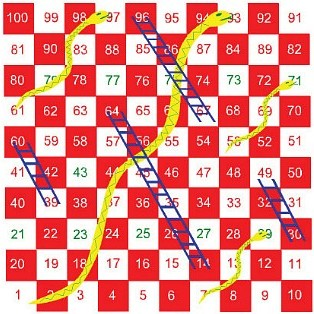
\includegraphics[scale=2.5]{images/SALboard}
\end{center}
\caption{The board that I will be studying.}
\end{figure}

\section{Markov Chains}
A Markov chain is a mathematical system that undergoes changes from one state to another. It is a random process in which the next state depends only on the current state and not on the sequence of events that preceded it. This is called the Markov property.

\section{Modelling the Game}
To model snakes and ladders I created a transition matrix. This is matrix where the value at position $[x,y]$ is the probability of moving from $x$ to $y$. The position $[0,0]$ is a players starting position (off the board). Below is the code used in sage to create the matrix.

\begin{verbatim}
a = matrix(QQ, 101) # creates a square matrix populated with 0's
ladders = [14, 30, 39, 67] # base of the ladders
snakes = [29, 71, 93, 97] # head of the snakes
snakesladders = snakes + ladders

def rolldice(N):
    """
    simulates the rolling of a dice
    Inputs: an integer N, the index of the row in the matrix
    Outputs: alter the matrix a to reflect the outcome of the dice
    """
    for i in range(1,7):
        try: # changes the next 6 values to 1/6.
            a[N, N + i] = 1/6
        except:
            pass

for k in range(101): # does rolldice over the entire matrix a.
    if k not in snakesladders:
        rolldice(k)

a[100,100] = 1 # when you get to 100, you win
a[29, 7] = 1 # snakes and ladders have a certain outcome
a[71, 53] = 1
a[93, 1] = 1
a[97, 61] = 1
a[14, 64] = 1
a[30, 49] = 1
a[39, 60] = 1
a[67, 96] = 1
\end{verbatim}

Then I created a vector to represent the probabilities of current position. It begins with just $1$ in $Row_0$ because the probability of being off the board at the start of the game is certain. By multiplying this vector by the transition matrix, it gets populated by more and more probabilities.

There is one big assumption made in this model though. It assumes that moving up/down a ladder/snake counts as a roll of the dice instead of being instantaneous. This is not how the game is normally played but the overall effect is small.

Where it does make a large difference is in computational speed. Matrix multiplication requires $n^3$ calculations and this particular board has a total of 8 ladders and snakes. If their corresponding rows and columns were removed from the transition matrix it would reduce the number of calculations required by $21.9\%$.

\bibliographystyle{plain}
\bibliography{SALbib}
\end{document}